\documentclass[tikz,border=10pt]{standalone}
\usepackage{amsmath}
\usepackage{amssymb}
\usepackage{tikz}
\usetikzlibrary{arrows.meta,calc,decorations.markings}

\definecolor{figazul}{RGB}{2,132,199}
\definecolor{figrojo}{RGB}{220,38,38}
\definecolor{figverde}{RGB}{22,163,74}

\begin{document}
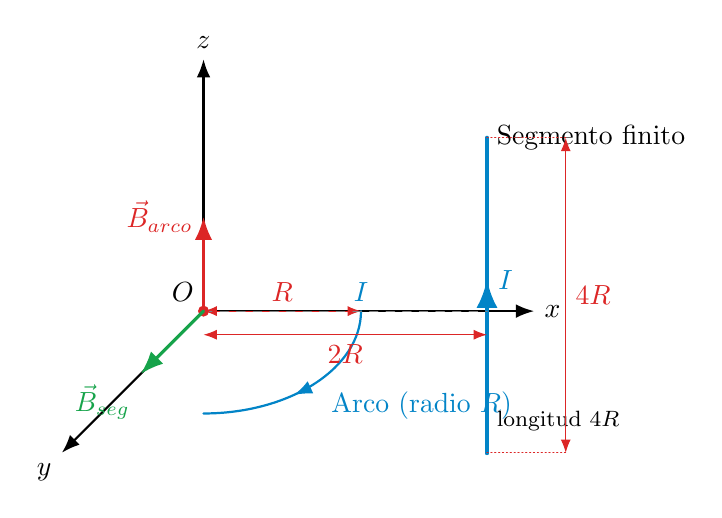
\begin{tikzpicture}[>=Latex, line cap=round, line join=round]
  % Ejes cartesianos en perspectiva
  \draw[->, thick] (0,0) -- (4.2,0) node[right] {$x$};
  \draw[->, thick] (0,0) -- (0,3.2) node[above] {$z$};
  \draw[->, thick] (0,0) -- (-1.8,-1.8) node[below left] {$y$};
  \node[above left] at (0,0) {$O$};

  % Radio R en escala
  % Arco en plano xy en 4to cuadrante: desde eje +x hacia eje -y
  % Coordenadas: x va de (1.8, 0) a (0, -1.8*projection)
  % En perspectiva: punto en x es (1.8, 0), punto en -y es (1.2, 1.2)
  % Dibujamos el plano xy con el arco
  \draw[thick, color=figazul, postaction={decorate, decoration={markings, mark=at position 0.55 with {\arrow{>}}}}]
    (2.0, 0) arc (0:-90:2.0 and 1.3);
  \node[above, color=figazul] at (2.0, 0) {$I$};
  \node[below right, color=figazul] at (1.5, -0.9) {Arco (radio $R$)};
  \draw[<->, thin, color=figrojo] (0,0) -- (2.0,0) node[midway, above, color=figrojo] {$R$};

  % Segmento finito paralelo a z en x = 2R (x = 4.0), y = 0
  \coordinate (SegBase) at (3.6, -1.8);
  \coordinate (SegTop) at (3.6, 2.2);
  \coordinate (SegMid) at (3.6, 0.2);

  \draw[ultra thick, color=figazul] (SegBase) -- (SegTop);
  \draw[->, ultra thick, color=figazul] (SegBase) -- ($(SegBase) + (0, 2.2)$) node[right, color=figazul] {$I$};
  \node[right] at (SegTop) {Segmento finito};
  \node[right, font=\footnotesize] at ($(SegBase) + (0, 0.4)$) {longitud $4R$};

  % Línea auxiliar desde O a la base del segmento en z = 0
  \draw[dashed, thin, color=gray] (0,0) -- (3.6,0);
  \draw[<->, thin, color=figrojo] (0,-0.3) -- (3.6,-0.3) node[midway, below, color=figrojo] {$2R$};

  % Cota vertical de longitud del segmento
  \draw[<->, thin, color=figrojo] (4.6, -1.8) -- (4.6, 2.2) node[midway, right, color=figrojo] {$4R$};
  \draw[densely dotted, thin, color=figrojo] (SegBase) -- (4.6, -1.8);
  \draw[densely dotted, thin, color=figrojo] (SegTop) -- (4.6, 2.2);

  % Campo resultante en el origen
  \fill[color=figrojo] (0,0) circle (2pt);
  \draw[->, very thick, color=figrojo] (0,0) -- (0, 1.2) node[left, color=figrojo] {$\vec{B}_{arco}$};
  \draw[->, very thick, color=figverde] (0,0) -- (-0.8, -0.8) node[below left, color=figverde] {$\vec{B}_{seg}$};
\end{tikzpicture}
\end{document}
